\documentclass[9pt]{beamer}

\usepackage{booktabs}
\usepackage{pifont}  % For checkmark and cross symbols
\usepackage{tikz}
\usetikzlibrary{shapes.geometric, arrows.meta, positioning, calc, patterns}
\usepackage{fontspec}
\usepackage{unicode-math}

\setmathfont{Latin Modern Math}

\usetheme{Madrid}
\usecolortheme{default}

\usepackage[
  backend=biber,
  style=apa,
  citestyle=apa,
  natbib=false,
  doi=false,
  isbn=false,
  url=false
]{biblatex}

\addbibresource{../shared/delivery_emission.bib}
\addbibresource{slides_local.bib}

\pdfstringdefDisableCommands{\def\dagger{*}\def\\{ }}
\usepackage{caption}
\setbeamertemplate{caption}[numbered]

\newcommand{\COtwoe}{CO\textsubscript{2}e}
\newcommand{\kgCOtwoe}{kg~\COtwoe}
\newcommand{\gCOtwoe}{g~\COtwoe}
\newcommand{\ktCOtwoe}{kt~\COtwoe}
\newcommand{\kgCOtwoePerKWh}{kg~\COtwoe~kWh$^{-1}$}
\newcommand{\kgCOtwoePerKg}{kg~\COtwoe~kg$^{-1}$}
\newcommand{\ktCOtwoePerYr}{kt~\COtwoe~yr$^{-1}$}

\title[Drone food delivery]{Road-network geometry and grid carbon intensity shape the climate mitigation benefits of drone food delivery across Chinese cities}


\author[Lin et al.]{\scriptsize Jingxian Lin\inst{1,*}, Jintao Ke\inst{1,*}, Xinglu Liu\inst{1}, Hongzheng Shi\inst{1},\\ Songhua Hu\inst{2}, Becky P. Y. Loo\inst{3}, Shuling Wang\inst{4},\\ Weiping Wang\inst{5,\dagger}, Klaus Hubacek\inst{6,\dagger}}
\institute[HKU, CityU, Tongji, Groningen]{\tiny
\inst{1} Department of Civil Engineering, The University of Hong Kong, Hong Kong, China\\
\inst{2} Department of Architecture and Civil Engineering, City University of Hong Kong, Hong Kong, China\\
\inst{3} Department of Geography, The University of Hong Kong, Hong Kong, China\\
\inst{4} Department of Traffic Information and Control Engineering, College of Transportation Engineering, Tongji University, Shanghai, China\\
\inst{5} Intelligent Robotic and Computational Perception Lab, Tongji University, Shanghai, China\\
\inst{6} Faculty of Science and Engineering, University of Groningen, Groningen, The Netherlands\\
\inst{*} Equal contribution. \inst{\dagger} Corresponding authors.}
\setbeamerfont{title}{size=\large}
\date[\today]{\today} % (optional)



\AtBeginSection[]
{
  \begin{frame}
    \frametitle{Table of Contents}
    \tableofcontents[currentsection]
  \end{frame}
}

\newcommand{\FlowchartColumn}[1]{%
  \begin{column}{0.35\textwidth}
    \begin{minipage}[c][.78\textheight][c]{\linewidth}
      \centering
      \resizebox{\linewidth}{!}{#1}
    \end{minipage}
  \end{column}
}

\newcommand{\ODFlowchart}{%
  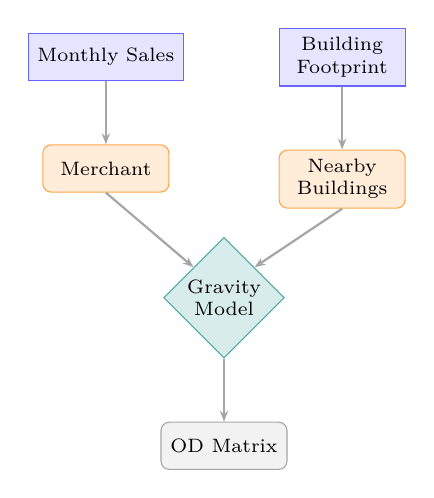
\begin{tikzpicture}[
      node distance=0.6cm and 1.2cm,
      data/.style={rectangle, draw=blue!60, fill=blue!10, minimum width=1.6cm, minimum height=0.6cm, align=center, font=\scriptsize},
      processed/.style={rectangle, draw=orange!70, fill=orange!15, rounded corners=3pt, minimum width=1.6cm, minimum height=0.6cm, align=center, font=\scriptsize},
      output/.style={rectangle, draw=gray!70, fill=gray!10, rounded corners=3pt, minimum width=1.6cm, minimum height=0.6cm, align=center, font=\scriptsize},
      model/.style={diamond, draw=teal!70, fill=teal!15, minimum width=1cm, minimum height=0.8cm, align=center, font=\scriptsize, inner sep=1pt},
      arrow/.style={-{Stealth[scale=0.6]}, thick, draw=gray!70}
    ]

    \node[data] (sales) {Monthly Sales};
    \node[data, right=1.2cm of sales] (building) {Building\\Footprint};

    \node[processed, below=0.8cm of sales] (merchant) {Merchant};
    \node[processed, below=0.8cm of building] (buildings) {Nearby\\Buildings};

    \path (merchant) -- (buildings) coordinate[midway] (mid);
    \node[model, below=0.8cm of mid] (gravity) {Gravity\\Model};

    \node[output, below=0.8cm of gravity] (od) {OD Matrix};

    \draw[arrow] (sales) -- (merchant);
    \draw[arrow] (building) -- (buildings);
    \draw[arrow] (gravity) -- (od);

    \draw[arrow] (merchant.south) -- (gravity.north west);
    \draw[arrow] (buildings.south) -- (gravity.north east);

  \end{tikzpicture}%
}

\newcommand{\RoadDistFlowchart}{%
  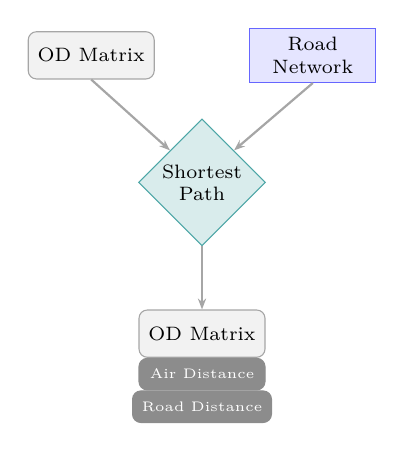
\begin{tikzpicture}[
      node distance=0.6cm and 1.2cm,
      data/.style={rectangle, draw=blue!60, fill=blue!10, minimum width=1.6cm, minimum height=0.6cm, align=center, font=\scriptsize},
      processed/.style={rectangle, draw=orange!70, fill=orange!15, rounded corners=3pt, minimum width=1.6cm, minimum height=0.6cm, align=center, font=\scriptsize},
      output/.style={rectangle, draw=gray!70, fill=gray!10, rounded corners=3pt, minimum width=1.6cm, minimum height=0.6cm, align=center, font=\scriptsize},
      smallbox/.style={rectangle, draw=gray!90, fill=gray!90, text=white, minimum width=1.6cm, minimum height=0.4cm, align=center, font=\tiny, rounded corners=3pt},
      model/.style={diamond, draw=teal!70, fill=teal!15, minimum width=1cm, minimum height=0.8cm, align=center, font=\scriptsize, inner sep=1pt},
      arrow/.style={-{Stealth[scale=0.6]}, thick, draw=gray!70}
    ]

    \node[output] (od) {OD Matrix};
    \node[data, right=1.2cm of od] (roadnet) {Road\\Network};

    \path (od) -- (roadnet) coordinate[midway] (mid);
    \node[model, below=0.8cm of mid] (shortest) {Shortest\\Path};

    \node[output, below=0.8cm of shortest] (result) {OD Matrix};

    \node[smallbox, below=0cm of result.south, anchor=north] (airdist) {Air Distance};
    \node[smallbox, below=0cm of airdist.south, anchor=north] (roaddist) {Road Distance};

    \draw[arrow] (shortest) -- (result);

    \draw[arrow] (od.south) -- (shortest.north west);
    \draw[arrow] (roadnet.south) -- (shortest.north east);

  \end{tikzpicture}%
}

\begin{document}

\frame{\titlepage}

\begin{frame}
  \frametitle{Table of Contents}
  \tableofcontents
\end{frame}

\section{Introduction}

\begin{frame}{Drone Delivery - An Emerging Industry}
  \begin{columns}[c]
    \begin{column}{0.58\textwidth}
      \begin{itemize}
        \item Drones are a \textbf{transformative technology} for transportation and logistics
        \item Key benefits:
          \begin{itemize}
            \item Fast and flexible delivery
            \item Cost-efficient operations
          \end{itemize}
        \item \textbf{Low-altitude economy} development gaining momentum in China
          \begin{itemize}
            \item Included in \textbf{China’s Government Work Report} in both 2024 and 2025, signaling sustained national-level policy attention
          \end{itemize}
        \item Global drone delivery market growth:
          \begin{itemize}
            \item US\$3.47~billion (2025) $\rightarrow$ US\$20.98~billion (2034)
            \item Compound Annual Growth Rate: \textbf{19.45\%}
          \end{itemize}
      \end{itemize}
    \end{column}
    \begin{column}{0.37\textwidth}
      \begin{figure}
        \centering
        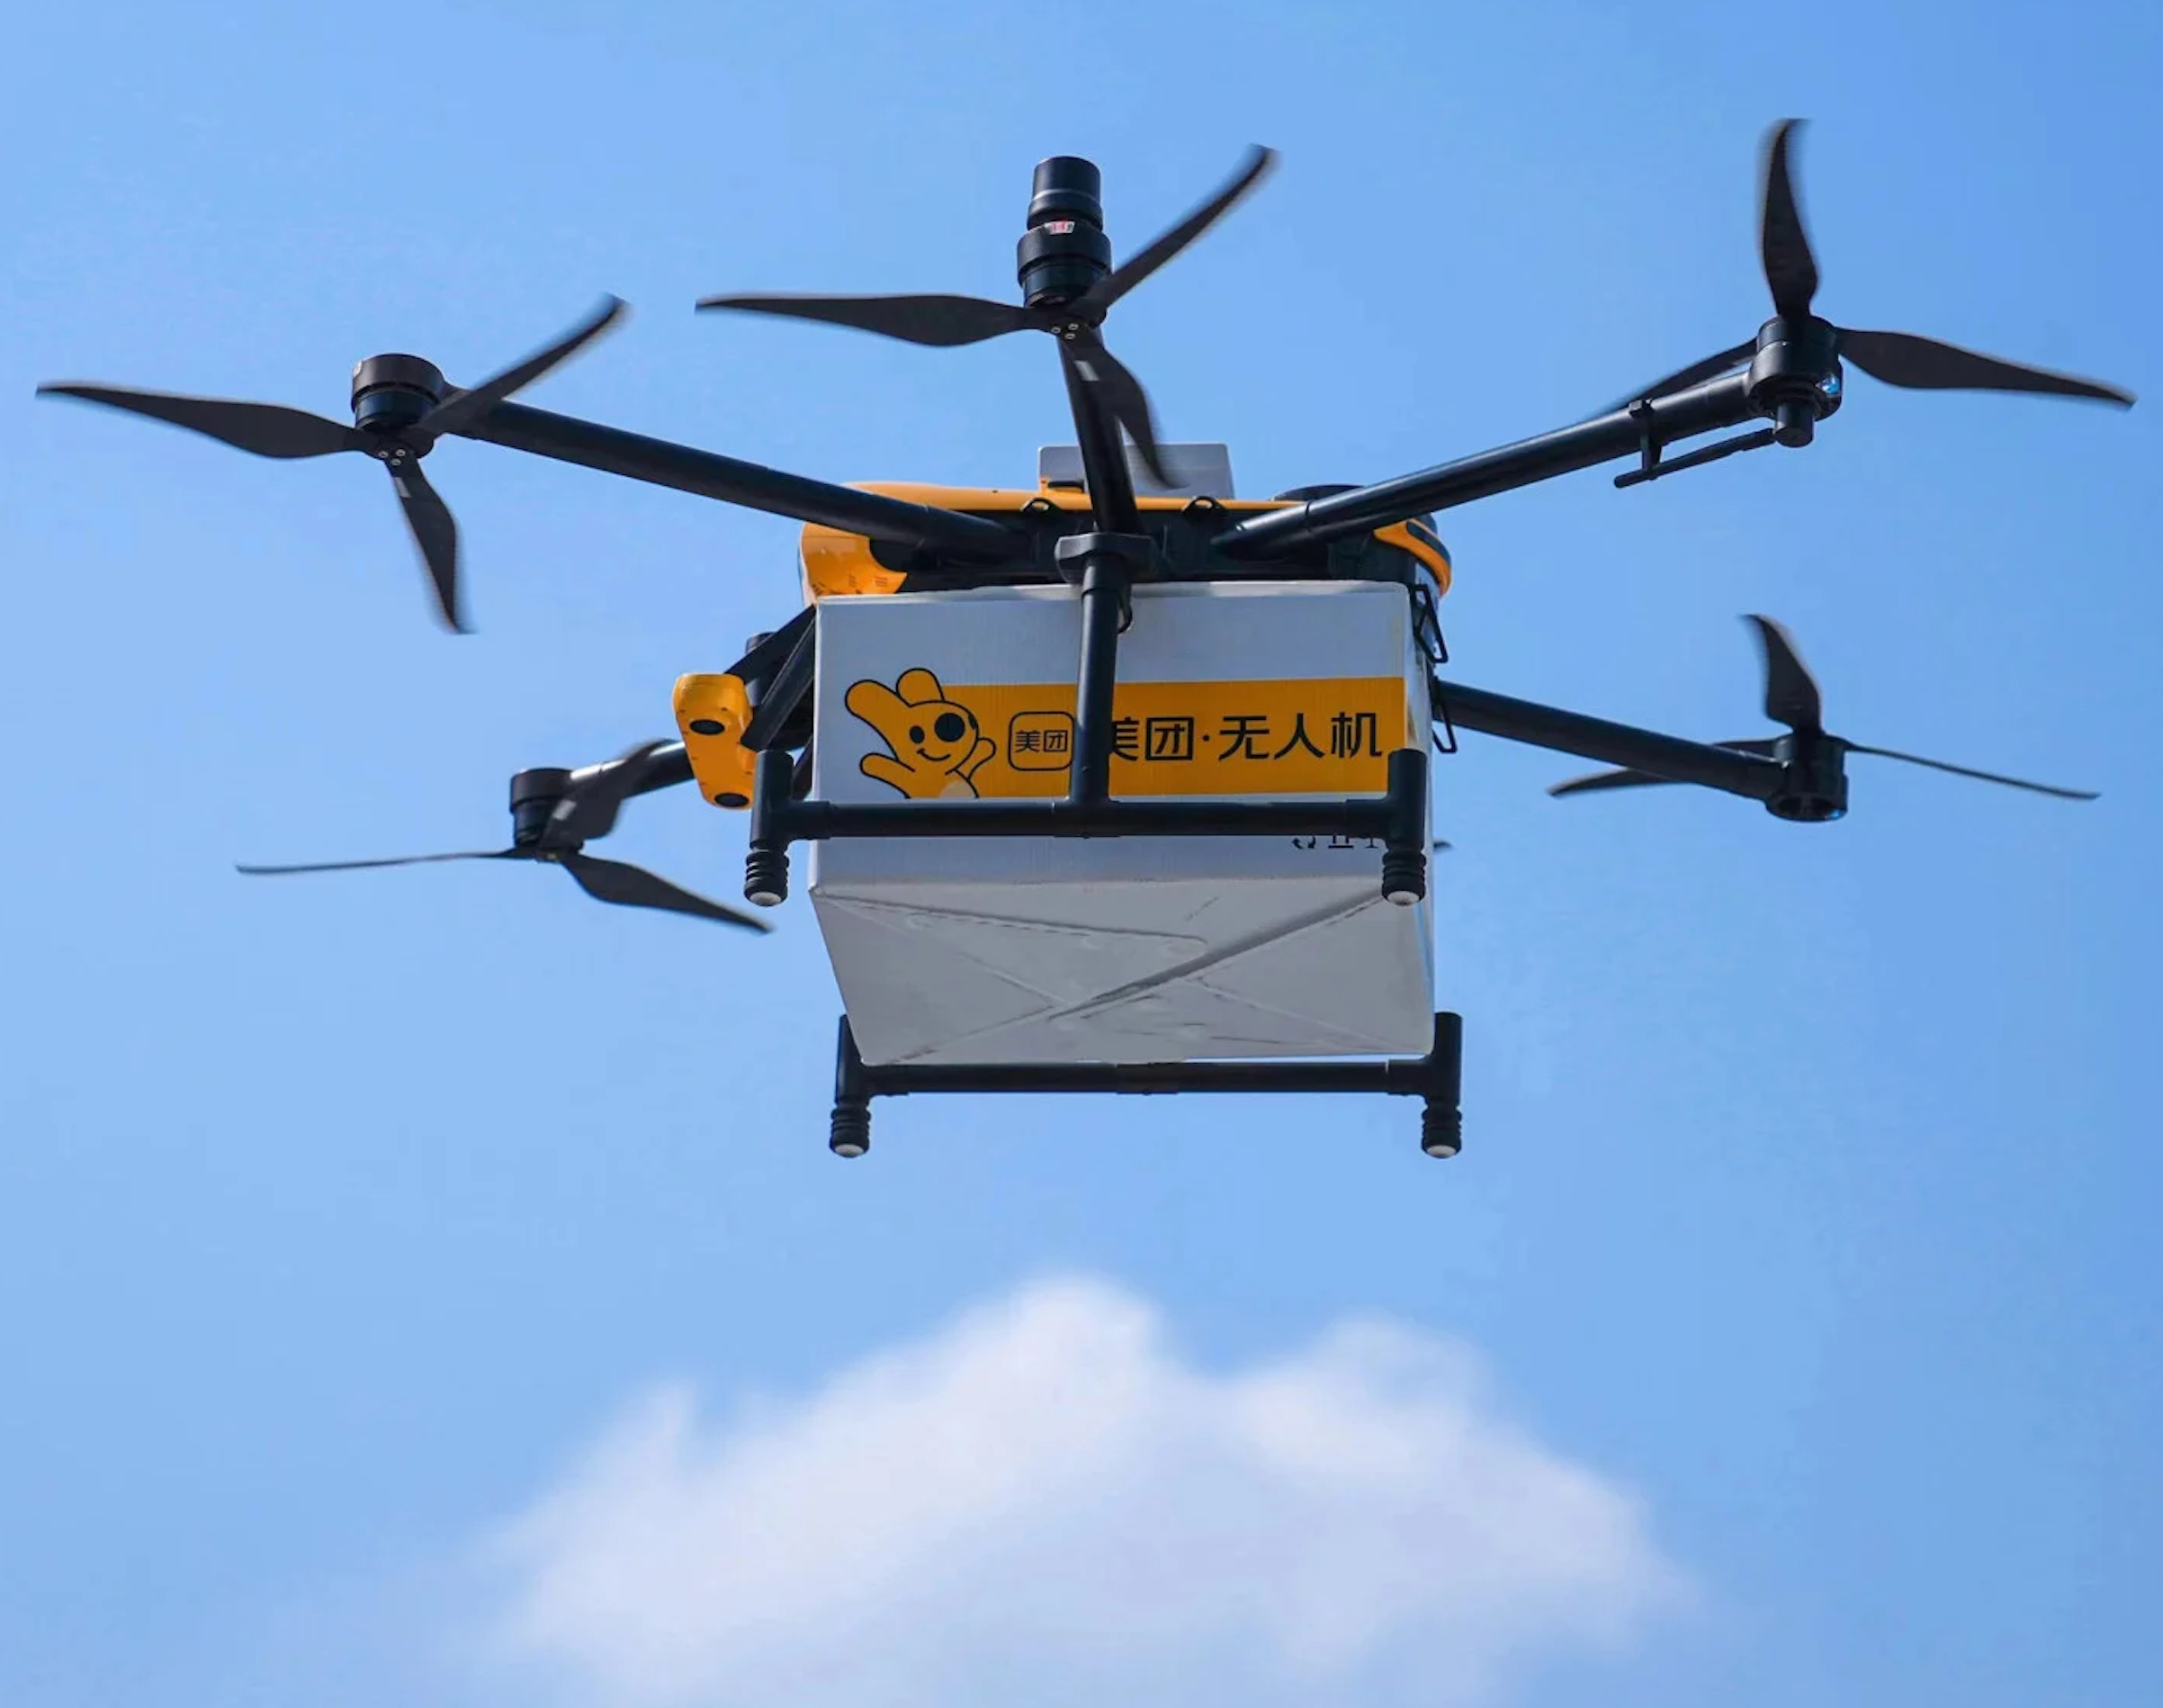
\includegraphics[width=\linewidth,height=0.64\textheight,keepaspectratio]{assets/Snipaste_2026-06-25_01-23-51.png}
        \caption{Meituan drone food delivery in operation.}
      \end{figure}
    \end{column}
  \end{columns}
\end{frame}

\begin{frame}{Why Food Delivery?}
  \begin{itemize}
    \item \textbf{Current constraints:} Battery capacity and cargo weight limitations
    \item Drones best suited for:
      \begin{itemize}
        \item Short-distance delivery
        \item Last-mile logistics
      \end{itemize}
    \item \textbf{Food delivery advantages} over parcel delivery:
      \begin{itemize}
        \item Lighter and smaller packages
        \item Shorter delivery distances (usually under 3~km)
        \item Speed advantage: prevents food from getting cold/spoiled
        \item High time sensitivity matches drone capabilities
      \end{itemize}
  \end{itemize}
\end{frame}

\begin{frame}{Food Delivery in China}
  \begin{columns}[c]
    \begin{column}{0.52\textwidth}
      \begin{figure}
        \centering
        \includegraphics[width=\linewidth]{assets/china_food_delivery_market_size.pdf}
        \caption{\textbf{China's online food delivery market size (2017--2027)} \parencite{statista2024chinafooddelivery}.}
        \label{fig:market_size}
      \end{figure}
    \end{column}
    \begin{column}{0.43\textwidth}
      \begin{itemize}
        \item Market expanded from approximately \textbf{300~billion yuan} in 2017 to over \textbf{1~trillion yuan} by 2023
        \item Large order volume creates substantial opportunity for drone adoption
        \item Leading platforms such as \textbf{Meituan} and \textbf{Eleme} have initiated pilot drone delivery programs in multiple cities
      \end{itemize}
    \end{column}
  \end{columns}
\end{frame}

\begin{frame}{Environmental Impact Remains Uncertain}
  \begin{itemize}
    \item The \textbf{environmental impact} of drone delivery systems remains uncertain
    \item Existing findings vary across comparison vehicles, geographic contexts, and methods
    \item \textbf{Lack of predictive emission models} across different urban contexts
    \item Unclear \textbf{when drones outperform conventional delivery} as a sustainable alternative
  \end{itemize}

\end{frame}

\begin{frame}{Review of Related Work}

  \footnotesize
  \centering
  \captionof{table}{Comparison of drone delivery emission studies}
  \resizebox{\linewidth}{!}{\begin{tabular}{l l c c c c}
    \toprule
    \textbf{Study} & \textbf{Comparison} & \textbf{Lower emissions?} & \textbf{OD Data} & \textbf{Scale} & \textbf{Method} \\
    \midrule
    \textcite{figliozzi_lifecycle_2017} & Van/Tricycle & Mixed & No & Analytical & LCA \\
    \textcite{park_comparative_2018} & Motorcycle & Yes & No & Two regions (Korea) & LCA \\
    \textcite{stolaroff_energy_2018} & Truck & Mixed & No & National (USA) & LCA \\
    \textcite{kirschstein_comparison_2020} & Truck & Mixed & No & Single city (Germany) & Use-phase \\
    \textcite{yowtak_comparative_2020} & ICEV/BEV & Mixed & No & Single city (USA) & LCA \\
    \textcite{baldisseri_truck-based_2022} & Truck & Yes & No & Suburban (Italy) & LCA \\
    \textcite{rodrigues_drone_2022} & Car/Van/Bike & Mixed & No & National (USA) & Use-phase \\
    \textcite{li_beyond_2025} & E-bike & Mixed & No & Single city (China) & LCA \\
    \midrule
    \textbf{This work} & \textbf{E-bike} & \textbf{Conditional} & \textbf{Modelled} & \textbf{313 cities (China)} & \textbf{LCA} \\
    \bottomrule
  \end{tabular}}
\end{frame}

\begin{frame}{Research Gaps in Prior Studies}
\begin{itemize}
  \item \textbf{Incumbent mode:} Asian food delivery relies heavily on e-bikes and bundled orders, creating an efficient ground baseline.
  \item \textbf{Destination coverage:} Nationwide merchant volumes are available, but nationwide observed customer destinations are missing.
  \item \textbf{Spatial variation:} Electricity supply and road detours jointly determine which trips favour drones.
\end{itemize}
\begin{block}{Research question}Under which city and trip conditions does selective drone substitution reduce lifecycle emissions?\end{block}
\end{frame}

\begin{frame}{Contributions}
\begin{itemize}
  \item We jointly calibrate a merchant-to-residential gravity model on observed Beijing orders, then reconstruct demand across \textbf{313 cities}.
  \item We compare lifecycle emissions using mode-specific routes, loaded outbound and empty return trips, and e-bike bundling.
  \item We quantify selective substitution, test city-specific road-distance thresholds, and examine grid, bundling and incumbent-mode scenarios.
\end{itemize}
\begin{block}{Data distinction}Merchant order volumes are observed. Nationwide destinations and OD flows are model generated.\end{block}
\end{frame}

\section{Method}

\begin{frame}{OD Generation - Overview}
\begin{columns}[c]
\FlowchartColumn{\ODFlowchart}
\begin{column}{0.60\textwidth}
\begin{itemize}
\item Observe merchant locations and August 2021 monthly order volumes.
\item Identify residential buildings within \textbf{5 km} of each merchant.
\item Jointly calibrate destination choice on observed Beijing OD orders.
\item Transfer parameters to \textbf{313 cities}: \textbf{398,270,072 modelled OD pairs}, representing \textbf{6,173,120,124 annualized orders}.
\item Annualization uses $P_i=12S_i$, assuming August represents an average month.
\end{itemize}
\end{column}
\end{columns}

\end{frame}

\begin{frame}{OD Generation - Monthly Sales Data}

  \begin{columns}[c]
    \FlowchartColumn{\ODFlowchart}
    \begin{column}{0.6\textwidth}
      \begin{figure}
        \centering
        \includegraphics[width=0.6\linewidth]{assets/screenshot.pdf}
        \caption{\textbf{Screenshot of the Meituan Takeaway app showing merchant information.} The dataset includes latitude, longitude, and monthly sales data for 1,075,362 merchants in the source dataset across China, collected in August 2021.}
        \label{fig:meituan_app}
      \end{figure}
    \end{column}
  \end{columns}

\end{frame}

\begin{frame}{OD Generation - Sales Heatmap}

  \begin{columns}[c]
    \FlowchartColumn{\ODFlowchart}
    \begin{column}{0.6\textwidth}
      \begin{figure}
        \centering
        \includegraphics[width=0.95\linewidth]{assets/shenzhen_heatmap.pdf}
        \caption{\textbf{Heatmap of the monthly sales data for Shenzhen.} The heatmap is generated using the latitude and longitude of the merchants and the monthly sales data.}
        \label{fig:shenzhen_heatmap}
      \end{figure}
    \end{column}
  \end{columns}

\end{frame}

\begin{frame}{OD Generation - Building Footprint Data}

  \begin{columns}[c]
    \FlowchartColumn{\ODFlowchart}
    \begin{column}{0.6\textwidth}
      \begin{figure}
        \centering
        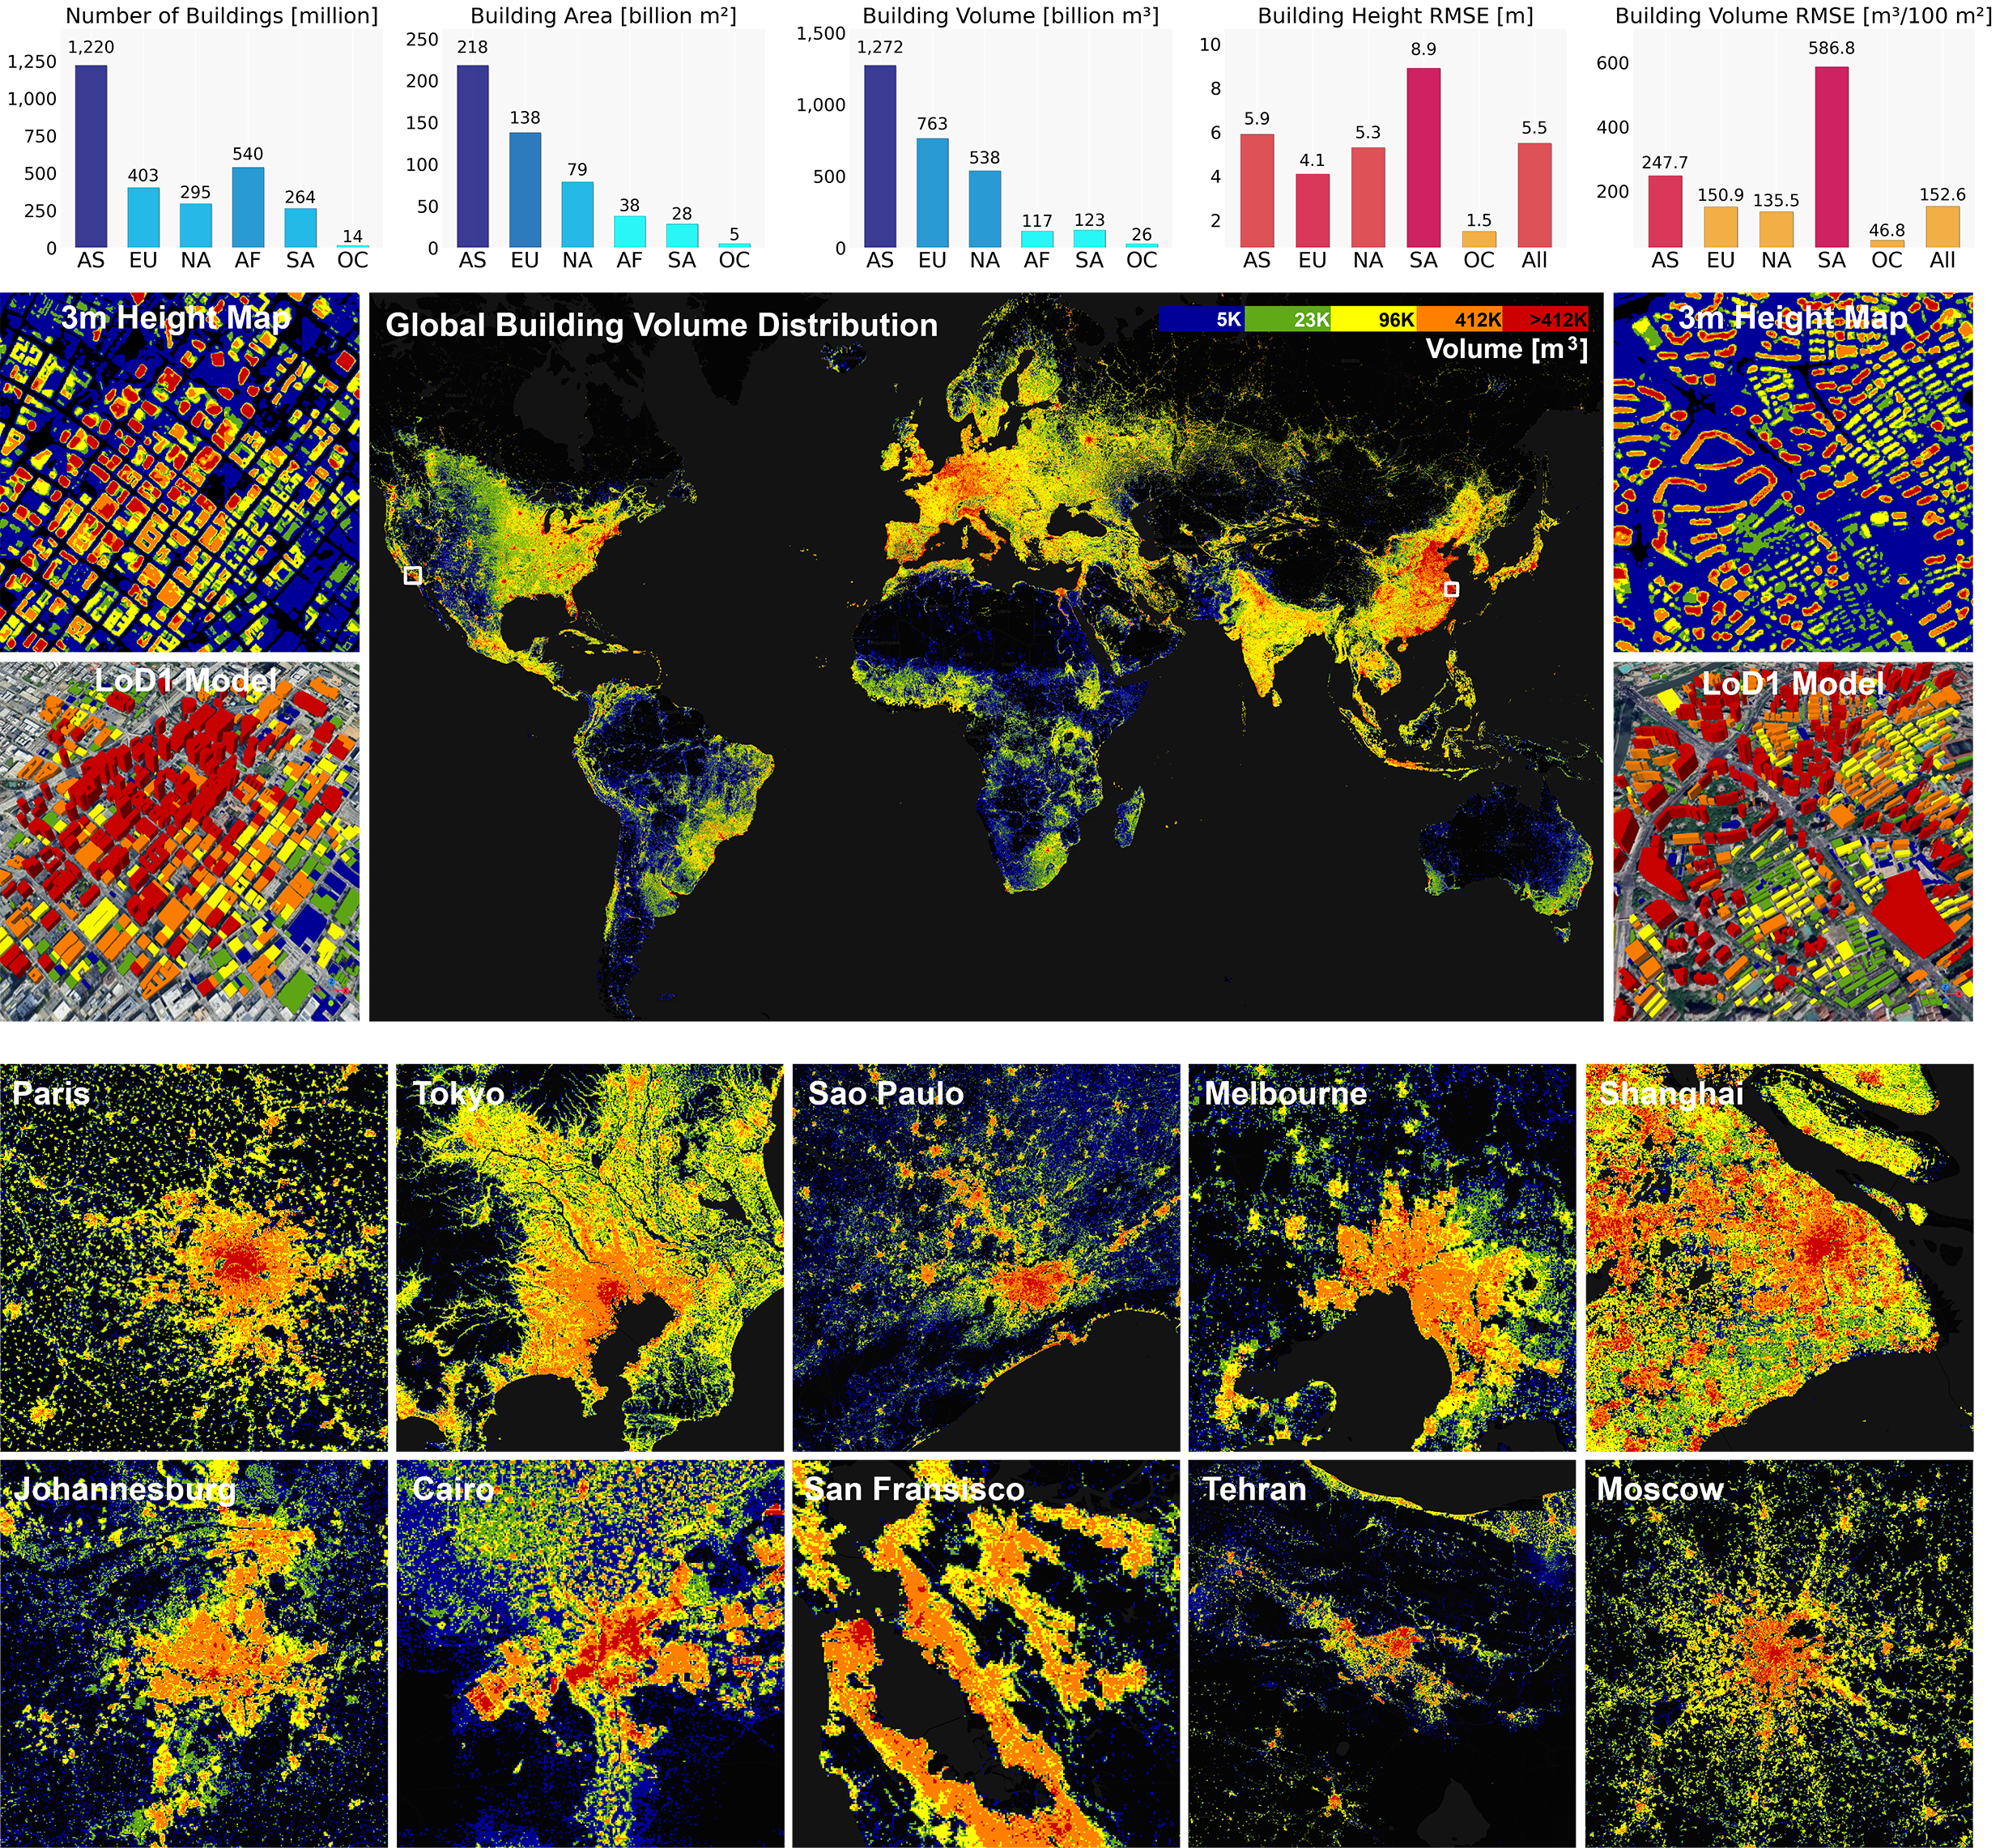
\includegraphics[width=0.8\linewidth]{assets/global_building_atlas.png}
        \caption{\textbf{Global Building Atlas}. The first open dataset providing global coverage of building polygons, heights, and LoD1 3D models, containing 2.75~billion buildings at 3~m resolution \parencite{zhu_globalbuildingatlas_2025}.}
        \label{fig:global_building_atlas}
      \end{figure}
    \end{column}
  \end{columns}

\end{frame}

\begin{frame}{OD Generation - Store Coverage}

  \begin{columns}[c]
    \FlowchartColumn{\ODFlowchart}
    \begin{column}{0.6\textwidth}
      \begin{figure}
        \centering
        \includegraphics[width=0.95\linewidth]{assets/shenzhen_store_coverage.pdf}
        \caption{\textbf{Building footprint data and store coverage for Shenzhen.} Nearby buildings are matched with takeout merchants as potential customers. Background illustration of the input geography. The current model considers residential destinations within 5 km of each merchant.}
        \label{fig:shenzhen_buildings}
      \end{figure}
    \end{column}
  \end{columns}

\end{frame}

\begin{frame}{OD Generation - Gravity Model}

  \begin{columns}[c]
    \FlowchartColumn{\ODFlowchart}
    \begin{column}{0.6\textwidth}
      Building volume is a proxy for destination attractiveness. The Tanner impedance function \parencite{tanner1961factors} represents the dependence of destination choice on merchant-to-building distance.
      \[
        D_{ij} = P_{i} \cdot \frac{f(d_{ij}, v_{j})}{\sum_{k \in \mathcal{D}_i} f(d_{ik}, v_{k})}, \quad \forall i \in \mathcal{O}, j \in \mathcal{D}_i
      \]

      where
      \[f(d_{ij}, v_{j}) = v_{j}^\alpha \cdot d_{ij}^{\beta} \cdot e^{-\gamma \cdot d_{ij}}.\]

      \footnotesize
      \centering
      \captionof{table}{Gravity model symbols and their descriptions}
      \begin{tabular}{c c}
        \toprule
        Symbol & Description \\
        \midrule
        $D_{ij}$ & Estimated deliveries from $i$ to $j$ \\
        $P_i$ & Total delivery demand at origin $i$ \\
        $d_{ij}$ & Distance from $i$ to $j$ \\
        $v_j$ & Building volume at destination $j$ \\
        $\alpha$ & Building volume elasticity \\
        $\beta, \gamma$ & Tanner impedance parameters \\
        $\mathcal{O}$ & Set of origins \\
        $\mathcal{D}_i$ & Buildings within 5 km of merchant $i$ \\
        \bottomrule
      \end{tabular}
    \end{column}
  \end{columns}

\end{frame}

\begin{frame}{OD Generation - Joint Model Calibration}
\[
p_{ij}=\frac{v_j^\alpha d_{ij}^{\beta}e^{-\gamma d_{ij}}}{\sum_{k\in\mathcal D_i}v_k^\alpha d_{ik}^{\beta}e^{-\gamma d_{ik}}},\qquad D_{ij}=12S_i p_{ij}
\]
\begin{itemize}
\item Jointly estimate $\alpha$, $\beta$ and $\gamma$ using observed Beijing OD orders and matched merchant/building distributions \parencite{tanner1961factors}.
\item Accepted fit: \textbf{$\alpha=0.422$, $\beta=0.326$, $\gamma=1.650$}, with distances in km.
\item Destination choice is conditional on each merchant's \textbf{5-km candidate set}.
\item Transfer to other cities assumes common destination-choice relationships. Merchant volumes and residential geography remain city specific.
\end{itemize}
\begin{block}{Evidence boundary}Beijing distribution checks do not validate destination allocation outside Beijing.\end{block}

\end{frame}

\begin{frame}{OD Generation - Observed and Modelled Distances}
\centering
\includegraphics[width=0.95\linewidth,height=0.48\textheight,keepaspectratio,trim=0 251 0 0,clip]{../paper/figures/extended_data_fig6_delivery_distance_distribution.pdf}
\vspace{0.3em}
\begin{minipage}{0.94\linewidth}
\footnotesize
\begin{itemize}
  \item \textbf{278,616 of 278,688} valid observed orders (99.97\%) are within 5 km.
  \item Bars use 0.2-km bins. The model histogram is conditional on the calibrated candidate set.
  \item Histogram weights are rescaled from 245,144 retained orders to 278,616 for visual comparison.
\end{itemize}
\end{minipage}
\par\raggedright\scriptsize\color{gray} Extended Data Fig.~5a

\end{frame}

\begin{frame}{OD Generation - Endpoint Distribution Check}
\centering
\includegraphics[width=0.95\linewidth,height=0.59\textheight,keepaspectratio,trim=0 0 0 160,clip]{../paper/figures/extended_data_fig6_delivery_distance_distribution.pdf}
\vspace{0.3em}
\begin{minipage}{0.94\linewidth}
\footnotesize
\begin{itemize}
  \item Observed and expected endpoint counts use aligned 1-km Beijing grids and a shared logarithmic colour scale.
  \item Each endpoint grid totals \textbf{245,144 orders}. This retained sample differs from the distance-coverage sample.
\end{itemize}
\end{minipage}
\par\raggedright\scriptsize\color{gray} Extended Data Fig.~5b

\end{frame}

\begin{frame}{Road Distance Calculation - Road Network}
  \begin{columns}[c]
    \FlowchartColumn{\RoadDistFlowchart}
    \begin{column}{0.6\textwidth}
      \begin{figure}
        \centering
        \includegraphics[width=0.7\linewidth]{assets/nanshan_roadnet.pdf}
        \caption{\textbf{Road network for the Nanshan district.} All road types except motorways are acquired from OpenStreetMap via the OSMnx library.}
        \label{fig:nanshan_roadnet}
      \end{figure}
    \end{column}
  \end{columns}
\end{frame}

\begin{frame}{Road Distance Calculation - Distance Comparison}
\centering
\includegraphics[width=0.95\linewidth,height=0.51\textheight,keepaspectratio,trim=395 385 0 0,clip]{../paper/figures/fig1_allocation_framework_national.pdf}
\vspace{0.3em}
\begin{minipage}{0.94\linewidth}
\footnotesize
\begin{itemize}
  \item Drone distance is the Haversine great-circle distance. E-bike distance is the shortest traversable road-network path.
  \item Trip detour: $\delta_n=d_n^{\mathrm{road}}/d_n^{\mathrm{air}}$. City detour: $\bar\delta_c=\sum q_n d_n^{\mathrm{road}}/\sum q_n d_n^{\mathrm{air}}$.
  \item Direct flight excludes air corridors and geofencing. Invalid road routes are excluded from analyses requiring road distance.
\end{itemize}
\end{minipage}
\par\raggedright\scriptsize\color{gray} Main Fig.~1a

\end{frame}


\begin{frame}{Power Consumption Components}
  \small
  \begin{center}
    \captionof{table}{Power consumption components represented in the use-phase model}
    \begin{tabular}{l l l}
      \toprule
      Mode & Component & Main driver \\
      \midrule
      Drone & Induced power & Lift and total weight \\
      Drone & Profile power & Rotor speed and blade drag \\
      Drone & Fuselage drag & Air density, frontal area, velocity \\
      Drone & Climb power & Payload, gravity, flight angle \\
      Drone & Auxiliary power & Onboard electronics \\
      \midrule
      E-bike & Rolling resistance & Mass, speed, road friction \\
      E-bike & Aerodynamic drag & Air density, frontal area, velocity \\
      E-bike & Grade resistance & Mass, speed, road slope \\
      E-bike & Acceleration power & Stop frequency and speed \\
      \bottomrule
    \end{tabular}
  \end{center}
\par\footnotesize Models adapted from \parencite{kirschstein_comparison_2020,stolaroff_energy_2018}.
\vspace{0.5em}
\par\scriptsize\color{gray} Technical details: \hyperlink{app:emission:1}{Appendix A1} and \hyperlink{app:emission:2}{A2}
\end{frame}

\begin{frame}{Round-trip Delivery Process}
\small
Both modes connect the same merchant and residential destination, with a loaded outbound journey and an empty return.
\vspace{0.5em}
\begin{center}
\captionof{table}{Round-trip delivery stages}
\renewcommand{\arraystretch}{1.35}
\begin{tabular}{@{}p{0.18\linewidth}p{0.30\linewidth}p{0.42\linewidth}@{}}
\toprule Stage & E-bike & Drone\\\midrule
Departure & Pickup and road departure & Loaded take-off\\
Outbound & Loaded road travel & Loaded aerial cruise\\
Delivery & Customer drop-off & Loaded landing and unloading hover\\
Return & Empty road travel & Empty take-off, return cruise and landing\\
\bottomrule
\end{tabular}
\end{center}
\begin{itemize}
\item Baseline payload: \textbf{1 kg} for both modes.
\item Drones serve one customer destination per flight. E-bike orders can share a bundled route.
\end{itemize}
\par\scriptsize\color{gray} Energy equations and operating parameters: \hyperlink{app:emission:3}{Appendix A3} and \hyperlink{app:emission:6}{A6}
\end{frame}

\begin{frame}{Lifecycle Emission Boundary}
\small
The comparison includes vehicle and battery production, delivery operation and end-of-life treatment.
\vspace{0.4em}
\begin{center}
\captionof{table}{Lifecycle components and per-order attribution}
\renewcommand{\arraystretch}{1.35}
\begin{tabular}{@{}p{0.18\linewidth}p{0.30\linewidth}p{0.42\linewidth}@{}}
\toprule Component & Included burden & Attribution to each order\\\midrule
Production & Vehicle body and batteries & Annualized inventory shared across modelled annual deliveries\\
Use phase & Electricity for the round trip & Trip energy combined with the local grid emission factor\\
End of life & Body and battery disposal & Annualized disposal burden shared across modelled annual deliveries\\
\bottomrule
\end{tabular}
\end{center}
\begin{itemize}
\item Travel distance and utilization affect the number of orders sharing embodied emissions.
\end{itemize}
\par\footnotesize\textbf{Model boundary:} The simplified drone throughput denominator omits take-off, landing and hover time.
\vspace{0.4em}
\par\scriptsize\color{gray} Inventory, allocation and approximation: \hyperlink{app:emission:4}{Appendix A4} and \hyperlink{app:emission:5}{A5}
\end{frame}

\begin{frame}{Bundling and Selective Assignment}
\textbf{E-bike bundling}
\begin{itemize}
\item Shared routes reduce the road distance attributed to each order, affecting both operational emissions and embodied-emission allocation.
\item Baseline coefficient: \textbf{$\kappa=0.769$}. It is a model-based conversion of observed Beijing bundle size, rather than a measured route-distance ratio \parencite{beardwood_shortest_1959}.
\end{itemize}
\vspace{0.4em}
\textbf{Mode assignment and aggregation}
\begin{itemize}
\item Assign an OD pair to a drone only when its lifecycle emissions are lower. Ties remain with e-bikes.
\item Weight each OD pair by its annualized order count to obtain city emissions, savings and drone share.
\item Compare the mixed fleet with the all-e-bike baseline. The ideal allocation excludes fleet, infrastructure and airspace constraints.
\end{itemize}
\par\scriptsize\color{gray} Bundling assumptions and allocation equations: \hyperlink{app:emission:6}{Appendix A6} and \hyperlink{app:emission:7}{A7}
\end{frame}

\section{Results}

\begin{frame}{Selective Allocation Framework}
\centering
\includegraphics[width=0.95\linewidth,height=0.58\textheight,keepaspectratio,trim=0 375 0 0,clip]{../paper/figures/fig1_allocation_framework_national.pdf}
\vspace{0.3em}
\begin{minipage}{0.94\linewidth}
\footnotesize
\begin{itemize}
  \item Observed merchant volumes and modelled residential destinations generate OD demand.
  \item Mode-specific routes, round-trip energy and lifecycle amortization determine the lower-emission mode.
\end{itemize}
\end{minipage}
\par\raggedright\scriptsize\color{gray} Main Fig.~1a
\end{frame}

\begin{frame}{Selective Deployment Reduces National Emissions by 15.66\%}
\centering
\includegraphics[width=0.95\linewidth,height=0.65\textheight,keepaspectratio,trim=0 0 0 232,clip]{../paper/figures/fig1_allocation_framework_national.pdf}
\vspace{0.3em}
\begin{minipage}{0.94\linewidth}
\footnotesize
\begin{itemize}
  \item \textbf{41.85 kt CO$_2$e/year} saved across 313 cities: \textbf{267.22 to 225.38 kt/year} relative to all-e-bike delivery.
  \item The representative Beijing trip is at the annual-order-weighted 75th percentile of road distance.
\end{itemize}
\end{minipage}
\par\raggedright\scriptsize\color{gray} Main Fig.~1b,c
\end{frame}

\begin{frame}{Absolute Mitigation Concentrates in Metropolitan Markets}
\centering
\includegraphics[width=0.95\linewidth,height=0.59\textheight,keepaspectratio,trim=0 175 175 0,clip]{../paper/figures/fig2_city_mitigation_priorities.pdf}
\vspace{0.3em}
\begin{minipage}{0.94\linewidth}
\footnotesize
\begin{itemize}
  \item Annual savings: Beijing \textbf{2.50 kt}, Guangzhou 2.38, Chongqing 1.72, Shenzhen 1.56, Chengdu 1.41 and Shanghai 1.35.
  \item Large delivery volumes create a larger pool of trips for selective substitution.
\end{itemize}
\end{minipage}
\par\raggedright\scriptsize\color{gray} Main Fig.~2a
\end{frame}

\begin{frame}{Relative Mitigation Is Largest in Southwestern Cities}
\centering
\includegraphics[width=0.95\linewidth,height=0.49\textheight,keepaspectratio,trim=0 0 0 258,clip]{../paper/figures/fig2_city_mitigation_priorities.pdf}
\vspace{0.3em}
\begin{minipage}{0.94\linewidth}
\footnotesize
\begin{itemize}
  \item Zhaotong reaches \textbf{48.30\%}. The other top-nine cities are in Yunnan or Sichuan (37.74--42.74\%).
  \item City median: \textbf{12.65\%}. Regional medians range from 8.49\% in the Northeast to 33.46\% in the Southwest.
\end{itemize}
\end{minipage}
\par\raggedright\scriptsize\color{gray} Main Fig.~2c
\end{frame}

\begin{frame}{Absolute and Percentage Reductions Define City Priorities}
\begin{columns}[c,totalwidth=\linewidth]
\begin{column}{0.46\textwidth}\centering
\includegraphics[width=\linewidth,height=0.72\textheight,keepaspectratio,trim=335 175 0 0,clip]{../paper/figures/fig2_city_mitigation_priorities.pdf}
\end{column}
\begin{column}{0.50\textwidth}\small
\begin{itemize}
  \item Median thresholds: \textbf{43.62 t CO$_2$e/year} and \textbf{12.65\%}.
  \item \textbf{99} highest-priority cities exceed both, \textbf{58} pilot candidates have high relative but smaller absolute savings, and \textbf{156} have lower relative benefits.
  \item These are exploratory climate priorities. Operational feasibility requires local assessment.
\end{itemize}
\end{column}
\end{columns}
\par\scriptsize\color{gray}Main Fig.~2b
\end{frame}

\begin{frame}{Population Correlates with Absolute Mitigation}
\centering
\includegraphics[width=0.95\linewidth,height=0.53\textheight,keepaspectratio,trim=0 0 0 0,clip]{../paper/figures/extended_data_fig1_population_reduction_contrast.pdf}
\vspace{0.3em}
\begin{minipage}{0.94\linewidth}
\footnotesize
\begin{itemize}
  \item Across 313 cities, population correlates with absolute savings: $r=0.813$ (95\% CI 0.772--0.848).
  \item Percentage savings show no clear association: $r=0.0496$ (95\% CI $-0.062$--0.160, $P=0.382$). This also does not establish equivalence.
\end{itemize}
\end{minipage}
\par\raggedright\scriptsize\color{gray} Extended Data Fig.~1
\end{frame}

\begin{frame}{Grid Carbon Intensity Changes the Lifecycle Balance}
\centering
\includegraphics[width=0.95\linewidth,height=0.57\textheight,keepaspectratio,trim=0 375 0 0,clip]{../paper/figures/fig4_gef_distance_detour.pdf}
\vspace{0.3em}
\begin{minipage}{0.94\linewidth}
\footnotesize
\begin{itemize}
  \item GEF 0.1--0.2 kg CO$_2$e/kWh: \textbf{18.8 g/order} for e-bikes and \textbf{12.1} for drones.
  \item GEF 0.7--0.8: \textbf{56.9} versus \textbf{57.5 g/order}. Higher flight electricity use can reverse the advantage.
\end{itemize}
\end{minipage}
\par\raggedright\scriptsize\color{gray} Main Fig.~3a,b
\end{frame}

\begin{frame}{Longer Trips Increasingly Favour Drones}
\centering
\includegraphics[width=0.95\linewidth,height=0.52\textheight,keepaspectratio,trim=0 201 0 270,clip]{../paper/figures/fig4_gef_distance_detour.pdf}
\vspace{0.3em}
\begin{minipage}{0.94\linewidth}
\footnotesize
\begin{itemize}
  \item Across the four city fits, each additional aerial kilometre raises e-bike-minus-drone lifecycle emissions by \textbf{4.87--10.47 g/order}.
  \item Longer trips dilute the fixed take-off and landing cost. Electricity and road geometry determine the city-specific advantage.
\end{itemize}
\end{minipage}
\par\raggedright\scriptsize\color{gray} Main Fig.~3c
\end{frame}

\begin{frame}{Road Detours Strengthen Benefits within Grid Groups}
\centering
\includegraphics[width=0.95\linewidth,height=0.52\textheight,keepaspectratio,trim=0 0 0 449,clip]{../paper/figures/fig4_gef_distance_detour.pdf}
\vspace{0.3em}
\begin{minipage}{0.94\linewidth}
\footnotesize
\begin{itemize}
  \item GEF groups: $\leq0.3$ kg CO$_2$e/kWh ($n=42$, $r=0.7583$) and $>0.3$ ($n=271$, $r=0.8835$).
  \item All 313 cities enter the analysis, including five with fallback GEFs. These descriptive associations do not isolate causal effects.
\end{itemize}
\end{minipage}
\par\raggedright\scriptsize\color{gray} Main Fig.~3d
\end{frame}

\begin{frame}{Electricity, Distance and Detour Define the Break-even Boundary}
\centering
\includegraphics[width=0.95\linewidth,height=0.65\textheight,keepaspectratio,trim=0 0 0 0,clip]{../paper/figures/extended_data_fig3_break_even_operating_envelope.pdf}
\vspace{0.3em}
\begin{minipage}{0.94\linewidth}
\footnotesize
\begin{itemize}
  \item Negative drone-minus-e-bike emissions favour drones. Cleaner electricity expands the favourable region.
  \item This idealized envelope explains model conditions. Local demand and flight constraints determine feasible use.
\end{itemize}
\end{minipage}
\par\raggedright\scriptsize\color{gray} Extended Data Fig.~3
\end{frame}

\begin{frame}{Avoided Road Operation Is the Largest Positive Contribution}
\centering
\includegraphics[width=0.92\linewidth,trim=0 366 145 28,clip]{../paper/figures/fig5_contribution_decomposition.pdf}
\par\vspace{0.4em}
\includegraphics[width=0.92\linewidth,trim=0 18 145 422,clip]{../paper/figures/fig5_contribution_decomposition.pdf}
\vspace{0.3em}
\begin{minipage}{0.94\linewidth}
\footnotesize
\begin{itemize}
  \item Relative to all-e-bike emissions: \textbf{+45.40 pp} avoided road operation, \textbf{+11.42 pp} embodied balance, \textbf{$-15.06$ pp} fixed flight and \textbf{$-26.11$ pp} cruise.
  \item Bundling is embedded in avoided road operation. Net national reduction: \textbf{15.66\%}.
\end{itemize}
\end{minipage}
\par\raggedright\scriptsize\color{gray} Main Fig.~4a, national and North China excerpt with original axes and legend
\end{frame}

\begin{frame}{City-specific Road-distance Rules}
\centering
\includegraphics[width=0.95\linewidth,height=0.63\textheight,keepaspectratio,trim=0 0 0 0,clip]{../paper/figures/fig4_road_distance_rule.pdf}
\vspace{0.3em}
\begin{minipage}{0.94\linewidth}
\footnotesize
\begin{itemize}
  \item Assign drones at $d_n^{\rm road}\geq d_c^*$. Thresholds range \textbf{0.03--2.37 km}, median \textbf{1.63 km}.
  \item City median reduction: \textbf{10.05\%} under the distance rule versus \textbf{12.65\%} under trip-level allocation. Paired median gap: \textbf{2.25 pp}.
  \item Retention: Chengdu 99.8\%, Guangzhou 93.6\%, Beijing 84.5\%, Shanghai 74.6\%. Independent dispatch validation remains necessary.
\end{itemize}
\end{minipage}
\par\raggedright\scriptsize\color{gray} Main Fig.~5

\end{frame}

\begin{frame}{Cleaner Electricity Expands Mitigation and Drone Share}
\centering
\includegraphics[width=0.84\linewidth,height=0.57\textheight,keepaspectratio,trim=0 329 52 0,clip]{../paper/figures/fig6_future_scenarios.pdf}
\hspace{0.02\linewidth}\includegraphics[width=0.065\linewidth,height=0.57\textheight,keepaspectratio,trim=550 65 0 63,clip]{../paper/figures/fig6_future_scenarios.pdf}
\vspace{0.3em}
\begin{minipage}{0.94\linewidth}
\footnotesize
\begin{itemize}
  \item Current selective allocation: \textbf{41.85 kt/year}, median city drone share \textbf{34.94\%}. Halved GEFs: \textbf{140.99 kt/year}, share \textbf{60.82\%}.
  \item Savings use the fixed current-grid, $\kappa=0.769$, all-e-bike reference and include grid decarbonization itself.
\end{itemize}
\end{minipage}
\par\raggedright\scriptsize\color{gray} Main Fig.~6a,b. Continuous 21-step pathway: Extended Data Fig.~4a. Shared colour scale: reduction relative to the fixed current anchor.
\end{frame}

\begin{frame}{Stronger Bundling Reduces the Role of Drones}
\centering
\includegraphics[width=0.84\linewidth,height=0.57\textheight,keepaspectratio,trim=0 0 52 318,clip]{../paper/figures/fig6_future_scenarios.pdf}
\hspace{0.02\linewidth}\includegraphics[width=0.065\linewidth,height=0.57\textheight,keepaspectratio,trim=550 65 0 63,clip]{../paper/figures/fig6_future_scenarios.pdf}
\vspace{0.3em}
\begin{minipage}{0.94\linewidth}
\footnotesize
\begin{itemize}
  \item $\kappa=0.65$: \textbf{60.70 kt/year} total savings and \textbf{19.41\%} median drone share. Combined with halved GEFs: \textbf{146.79 kt/year} and \textbf{38.22\%}.
  \item All savings use the same fixed current all-e-bike anchor. They include bundling and grid benefits, rather than isolating drones.
\end{itemize}
\end{minipage}
\par\raggedright\scriptsize\color{gray} Main Fig.~6c,d. Continuous 21-step pathway: Extended Data Fig.~4b. Shared colour scale: reduction relative to the fixed current anchor.
\end{frame}

\begin{frame}{Lifecycle Comparison of Five Delivery Modes}
\centering
\includegraphics[width=0.95\linewidth,height=0.53\textheight,keepaspectratio,trim=0 280 0 0,clip]{../paper/figures/fig7_delivery_mode_lifecycle_comparison.pdf}
\vspace{0.3em}
\begin{minipage}{0.94\linewidth}
\footnotesize
\begin{itemize}
  \item Beijing, common one-way travelled distance \textbf{2.2235 km}, GEF 0.558 kg CO$_2$e/kWh, one unbundled order per round trip.
  \item Drone \textbf{84.0}, e-bike \textbf{83.5}, fuel moped \textbf{292.6}, electric car \textbf{750.2}, fuel car \textbf{1,060.6 g CO$_2$e/order}.
  \item Holding travel distance equal removes the aerial-route advantage present in Main Fig.~1b.
\end{itemize}
\end{minipage}
\par\raggedright\scriptsize\color{gray} Main Fig.~7a. Inventory source: \parencite{itf_good_to_go_2020}.
\end{frame}

\begin{frame}{Four-city Mitigation Depends on the Incumbent Mode}
\centering
\includegraphics[width=0.95\linewidth,height=0.64\textheight,keepaspectratio,trim=0 0 0 188,clip]{../paper/figures/fig7_delivery_mode_lifecycle_comparison.pdf}
\vspace{0.3em}
\begin{minipage}{0.94\linewidth}
\footnotesize
\begin{itemize}
  \item Mode-specific routes and $\kappa=0.769$: reductions of \textbf{10.2--34.5\%} against e-bikes, \textbf{67.8--91.9\%} against mopeds, \textbf{87.8--94.0\%} against electric cars and \textbf{91.1--97.8\%} against fuel cars.
  \item Drone share: \textbf{31.4--95.0\%} against e-bikes, \textbf{96.8--99.7\%} against mopeds, and above \textbf{99.5\%} against either car baseline.
\end{itemize}
\end{minipage}
\par\raggedright\scriptsize\color{gray} Main Fig.~7b,c. Each incumbent mode supplies its own lifecycle baseline.
\end{frame}

\section{Discussion}

\begin{frame}{Robustness of the Fixed Distance Strategy}
\centering
\includegraphics[width=0.95\linewidth,height=0.59\textheight,keepaspectratio,trim=0 0 0 0,clip]{../paper/figures/candidate_probability_positive_reduction_maps.pdf}
\vspace{0.3em}
\begin{minipage}{0.94\linewidth}
\footnotesize
\begin{itemize}
  \item \textbf{17 parameters}, triangular distributions, \textbf{10,000 draws per city}. Baseline thresholds and mode assignments stay fixed.
  \item Recalculate mixed-system and all-e-bike emissions in each draw. Median probability of positive mitigation: \textbf{0.8110 independent}, \textbf{0.6745 correlated adverse stress}.
  \item These are parameter-robustness probabilities for the fixed policy, rather than observed deployment success rates.
\end{itemize}
\end{minipage}
\par\raggedright\scriptsize\color{gray} Extended Data Fig.~2

\end{frame}

\begin{frame}{Selective Deployment and Model Boundaries}
\begin{itemize}
  \item Prioritize cities using absolute and percentage mitigation, then test local demand coverage and operational feasibility.
  \item Beijing-calibrated demand and bundling transfer nationally. Payload is fixed at 1 kg.
  \item Weather, airspace, fleet capacity, infrastructure, noise, safety and privacy can constrain deployment. Annual GEFs omit marginal and time-of-day emissions.
  \item \textbf{Potential heat benefit:} Replacing rider-operated trips could reduce occupational heat exposure. This benefit is \textbf{not quantified} here.
\end{itemize}
\begin{block}{Implication}Drones can complement bundled e-bikes on suitable trips. Dispatch should minimize emissions from the complete delivery system.\end{block}
\end{frame}

\section{References}

\begin{frame}[allowframebreaks]{References}
  \printbibliography
\end{frame}


\pdfstringdefDisableCommands{\def\translate#1{#1}}
\appendix
\AtBeginSection[]{}
\section*{Appendix}
\begin{frame}{Appendix: Emission Model Details}
\begin{itemize}
\item A1--A2: Mode-specific power models
\item A3: Round-trip energy and grid factors
\item A4--A5: Lifecycle inventory and throughput
\item A6--A7: Vehicle parameters, bundling and allocation
\end{itemize}
\end{frame}

\begin{frame}{Appendix A1: E-bike Power Model}
\label{app:emission:1}
\small
Rolling resistance, road grade, drag and acceleration enter the implemented power expression \parencite{kirschstein_comparison_2020}:
\[
P_E=m_tg(C_{\rm rr}+i)v+\frac{\rho C_dAv^3}{2000}
+\frac{n_{\rm acc}\,0.504\,v_h^3m_t}{2\times1000\times3.6}.
\]
\begin{itemize}
\item $P_E$ in kW, $m_t=m/1000$ in tonnes, $v$ in m/s and $v_h=3.6v$ in km/h.
\item Outbound mass includes body, batteries, rider and payload. Return mass excludes payload.
\item The road-grade term applies to both directions as an aggregate resistance assumption.
\item No separate auxiliary-power term enters the active e-bike expression.
\end{itemize}
\[
E^E_n=(P_{E,\rm out}+P_{E,\rm ret})\kappa d_n^{\rm road}/v_h\quad\text{(kWh/order)}.
\]

\end{frame}

\begin{frame}{Appendix A2: Drone Power Model}
\label{app:emission:2}
\small
Induced, profile, drag, climb and auxiliary terms enter the multirotor power model \parencite{kirschstein_comparison_2020,stolaroff_energy_2018}:
\[
P_D=\frac{k_{\rm lift}Tw+Dv+mgv\sin\theta}{1000}
+\frac{\rho R U^3[1+3(v/U)^2]\sigma C_{d,\rm blade}}{8000}+P_{\rm aux}.
\]
\[
T=\sqrt{(mg)^2+D^2+2Dmg\sin\theta},\quad
w^4-2v\sin\phi\,w^3+v^2w^2-\left(\frac{T}{2\rho R}\right)^2=0.
\]
\begin{itemize}
\item $w$ is the smallest positive real induced-velocity solution. At hover, $T=mg$ and $w=\sqrt{T/(2\rho R)}$.
\item $R=N_r\pi r^2$, $\sigma=N_b\bar c/(\pi r)$, and $U=\sqrt{6m_0g/(\rho N_rN_b\bar c C_l r)}$.
\item $\phi=\arctan[(-D-mg\sin\theta)/(mg\cos\theta)]$ for $v>0$.
\item Headwind alters body drag, but does not alter ground travel time.
\end{itemize}

\end{frame}

\begin{frame}{Appendix A3: Round-trip Energy and Grid Factors}
\label{app:emission:3}
\small
\[
E^E_n=(P_{E,\rm out}+P_{E,\rm ret})\kappa d_n^{\rm road}/v_E
\]
\[
\begin{aligned}
E^D_n={}&P_{\rm to,out}t_{\rm to}+P_{\rm cruise,out}t_{\rm cruise,out}
+P_{\rm land,out}t_{\rm land}+P_{\rm hover}t_{\rm hover}\\
&+P_{\rm to,ret}t_{\rm to}+P_{\rm cruise,ret}t_{\rm cruise,ret}
+P_{\rm land,ret}t_{\rm land}.
\end{aligned}
\]
\begin{itemize}
\item Drone: loaded take-off, outbound cruise, loaded landing and unloading hover, then empty take-off, return cruise and empty landing.
\item Vertical-phase time: $h/(1000v_{\rm vertical})$ h. Cruise time: $d^{\rm air}/v_{\rm cruise}$ h. Hover: $t_{\rm hover}/3600$ h.
\item Use-phase emissions are $E_n^m\mathrm{GEF}_c$ for each mode $m$.
\item Provincial GEFs span 0.107--0.725 kg CO$_2$e/kWh. Five cities use the national fallback, 0.5366 \parencite{mee_gef_2024}.
\end{itemize}

\end{frame}

\begin{frame}{Appendix A4: Lifecycle Inventory and Amortization}
\label{app:emission:4}
\small
Body and battery emissions are annualized separately:
\[
A_m=\frac{m_b(e_{\rm body}+e_{\rm body,EOL})}{L_v}
+\frac{C_b(e_{\rm battery}+e_{\rm battery,EOL})}{L_b}.
\]
\[
\ell_n^m=E_n^m\mathrm{GEF}_c+A_m/N_{m,n},\qquad N_{m,n}=60HD_yu/\tau_{m,n}.
\]
\centering
\begin{tabular}{lrr}
\toprule Assumption & E-bike & Drone\\\midrule
Body mass (kg) & 55 & 10.1\\
Installed battery capacity (kWh) & 1.20 & 1.556\\
Vehicle / battery life (years) & 4 / 2 & 4 / 2\\
Operating hours (h/day) & 8 & 12\\
Operating days (days/year) & 300 & 300\\
Loading time (min/order) & 3 & 0.5\\
\bottomrule
\end{tabular}
\par\raggedright\footnotesize Continuous battery amortization avoids integer rounding of replacements. Production and end-of-life factors apply separately.

\end{frame}

\begin{frame}{Appendix A5: Distance-dependent Throughput}
\label{app:emission:5}
\[
\tau_{E,n}=120\kappa d_n^{\rm road}/v_E+t_{E,\rm load},\qquad
\tau_{D,n}=120d_n^{\rm air}/v_D+t_{D,\rm load}.
\]
\begin{itemize}
\item Cycle times are in minutes, distances in km, and speeds in km/h.
\item Embodied emissions per order depend on OD distance through annual throughput $N_{m,n}$.
\item E-bike bundling affects both operational distance and amortization throughput. There is no additional division by mean bundle size.
\item Drone vertical-flight and hover energy enter use-phase emissions, but their durations are excluded from the simplified throughput denominator.
\end{itemize}
\begin{block}{Model boundary}Omitting vertical and hover time from throughput increases assumed annual deliveries relative to a full flight-cycle denominator.\end{block}

\end{frame}

\begin{frame}{Appendix A6: Vehicle Parameters and Bundling}
\label{app:emission:6}
\small
\begin{columns}[T]
\begin{column}{0.48\textwidth}
\begin{tabular}{lrr}
\toprule Parameter & E-bike & Drone\\\midrule
Loaded mass (kg) & 156 & 14.1\\
Empty mass (kg) & 155 & 13.1\\
Payload (kg) & 1 & 1\\
Speed (km/h) & 30 & 60\\
Vertical speed (km/h) & --- & 20\\
Take-off height (m) & --- & 100\\
Loaded hover (s) & --- & 10\\
\bottomrule
\end{tabular}
\end{column}
\begin{column}{0.48\textwidth}
\begin{itemize}
\item Beijing mean bundle size: $\bar B=1.69$.
\item Approximation: $\kappa=1/\sqrt{\bar B}=0.769$ \parencite{beardwood_shortest_1959}.
\item $\kappa$ converts bundle size to attributed distance. It is not a measured route-distance ratio.
\item Transfer nationally assumes common mean bundling efficiency.
\end{itemize}
\end{column}
\end{columns}
\end{frame}

\begin{frame}{Appendix A7: Assignment and City Aggregation}
\label{app:emission:7}
\[
z_n=\begin{cases}1,&\ell_n^D<\ell_n^E,\\0,&\ell_n^D\geq\ell_n^E,\end{cases}
\qquad G_c^{\rm mixed}=\sum_{n\in c}q_n[z_n\ell_n^D+(1-z_n)\ell_n^E].
\]
\[
G_c^E=\sum_{n\in c}q_n\ell_n^E,\quad A_c=G_c^E-G_c^{\rm mixed},\quad
R_c=100A_c/G_c^E.
\]
\begin{itemize}
\item Assign drones only when their lifecycle emissions are lower. Ties remain with e-bikes.
\item $q_n$ is the modelled annual order count. Drone share is $\sum q_nz_n/\sum q_n$.
\item This ideal benchmark excludes fleet, infrastructure and airspace constraints.
\end{itemize}
\end{frame}

\end{document}

